% Slides for 2025-08-19
% To create a slide, use the following:
% \begin{frame}{TITLE}
%     BODY
% \end{frame}

% To create a slide with a bullet list, use the following:
% \begin{frame}{TITLE}
%     \begin{itemize}
%         \item ITEM 1
%         \item ITEM 2
%     \end{itemize}    
% \end{frame}

% To create a slide with numbered list, use the following:
% \begin{frame}{TITLE}
%     \begin{enumerate}
%         \item ITEM 1
%         \item ITEM 2
%     \end{enumerate}
% \end{frame}

% To create a slide with a graphic:
% 1. Add the graphic to this folder (named picture.png)
% 2. Use the following:
% \begin{frame}{TITLE}
%     \centering
%     \includegraphics[height=0.7\textheight,width=0.7\textwidth,keepaspectratio]{picture.png}
% \end{frame}

% To create a slide with two columns, use the following:
% \begin{frame}{TITLE}
%     \begin{columns}
%         \begin{column}{0.5\textwidth}
%             COLUMN 1 BODY
%         \end{column}
%         \begin{column}{0.5\textwidth}
%             COLUMN 2 BODY
%         \end{column}
%     \end{columns}
% \end{frame}

\begin{frame}{ArcGIS Tool}
    \centering
    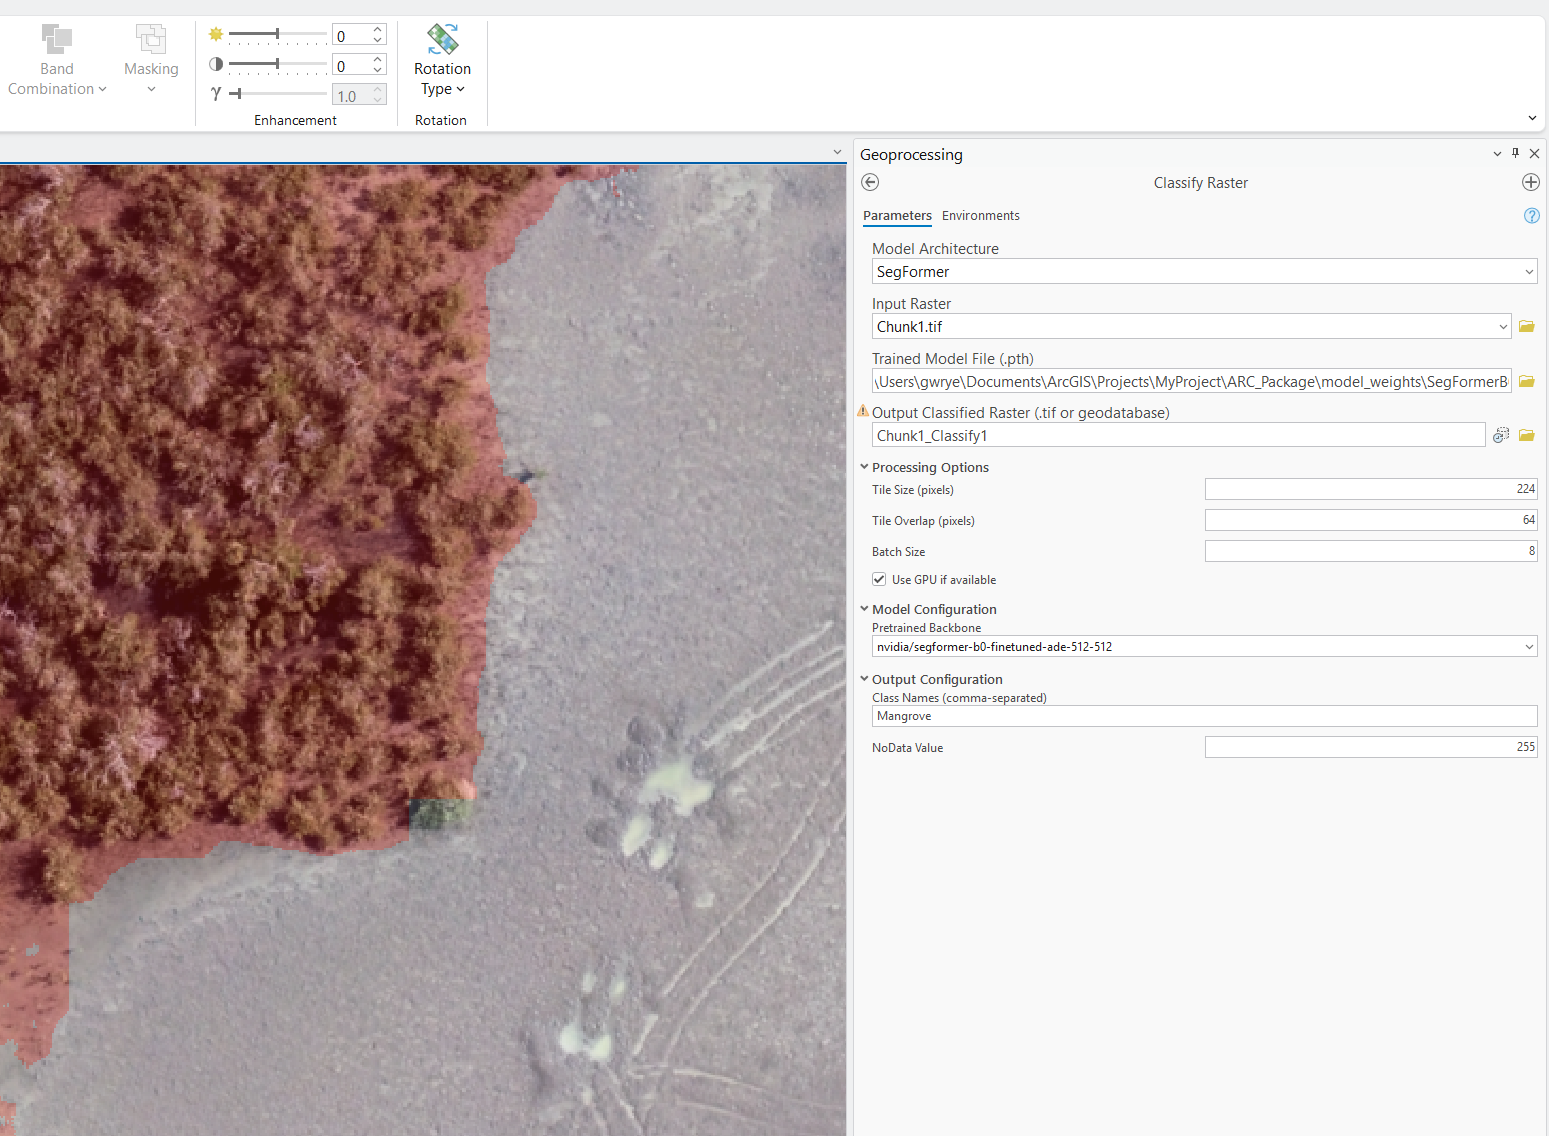
\includegraphics[height=0.7\textheight,width=0.7\textwidth,keepaspectratio]{images/arcgis.png}
\end{frame}

\begin{frame}{End-to-End ML Pipeline Completed}
    \vspace{1em}
    \centering
    GeoTiff $\rightarrow$ Dataset Creation $\rightarrow$ Model Training $\rightarrow$ ArcGIS Deployment
    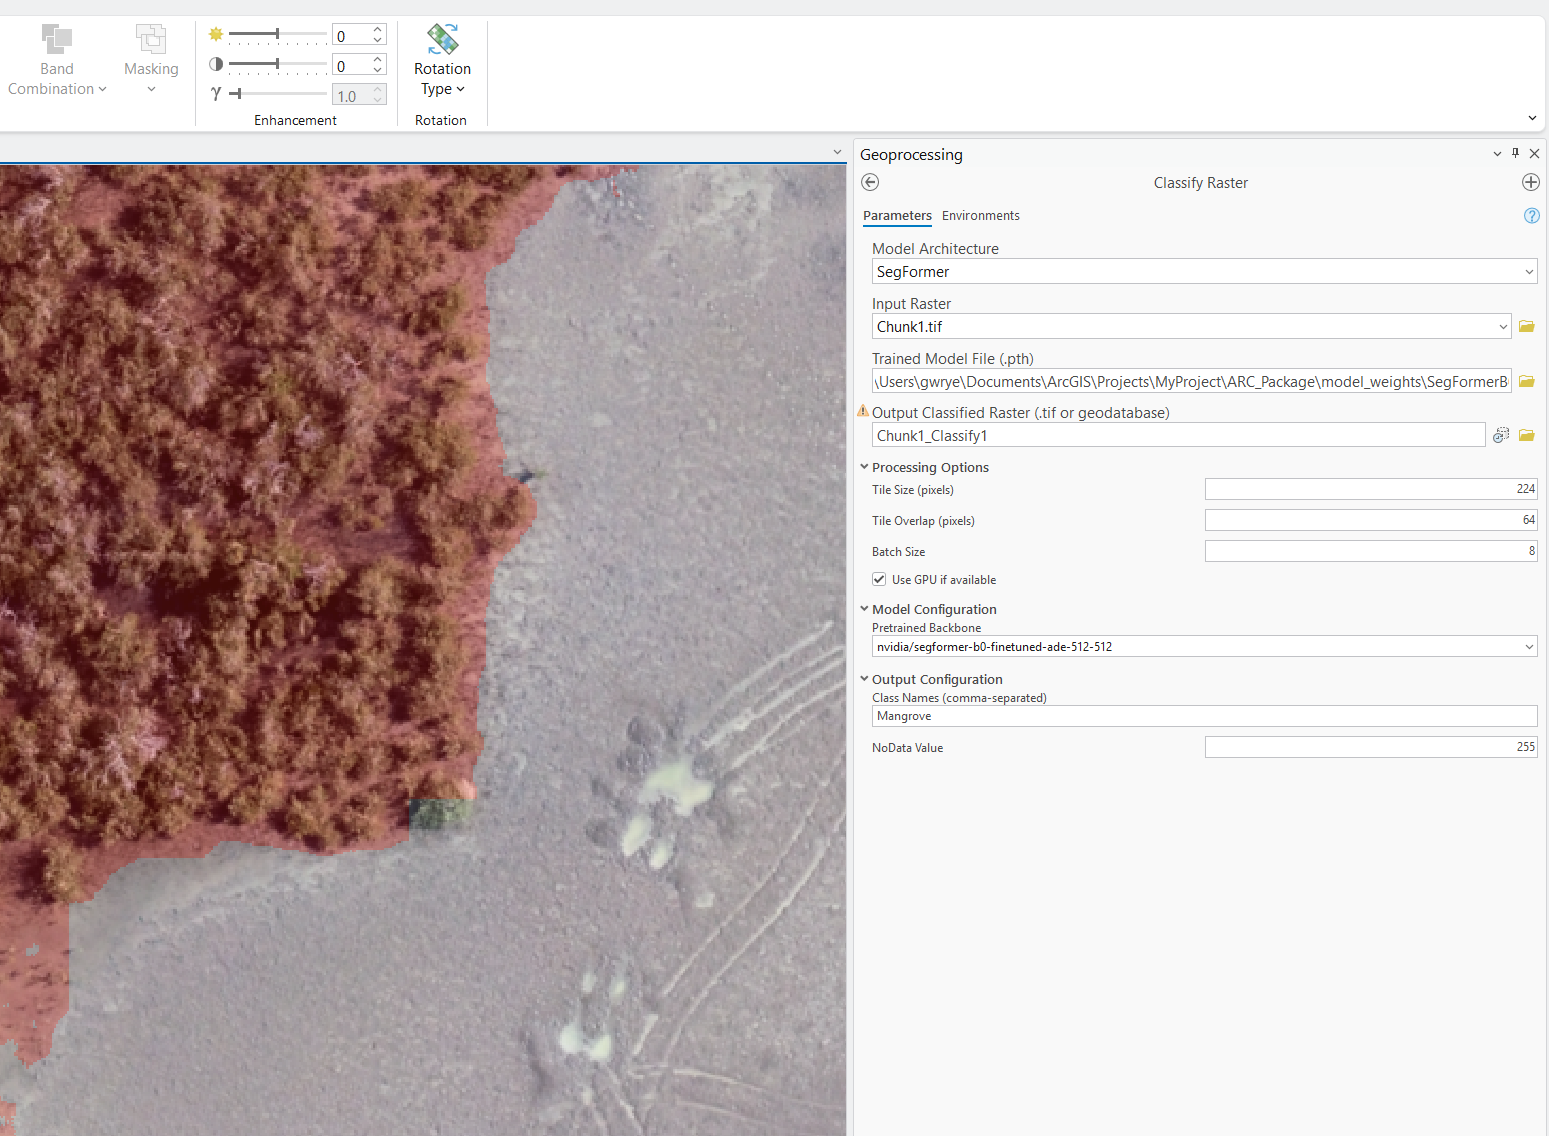
\includegraphics[height=0.7\textheight,width=0.7\textwidth,keepaspectratio]{images/arcgis.png}
\end{frame}

\begin{frame}{Small Data Processing Optimization}
    \begin{itemize}
        \item Made optimization to GeoTiff $\rightarrow$ Dataset pipeline, improving asymptotic runtime from $O(n^2)$ to $O(n)$ for number of tiles $n$
        \item Stores temporary, batch-wise image/label files and collects everything at the end instead of modifying the memory mapped array periodically
    \end{itemize}
\end{frame}

\begin{frame}{Next Steps}
    \begin{itemize}
        \item Show SIO team the ArcGIS tool
        \item Get Feedback on models and tool
        \item Create human infrastructure identification model
    \end{itemize}
\end{frame}